\subsection{PetaLinux}
\label{subsec:embedded_platform:operating_systems:petalinux}

Xilinx provides PetaLinux Tools to build your own PetaLinux \acrshort{os}.
It is recommended to work with the so-called target platform.
The target platform is a combination of hardware and software components.
The most important hardware component is a proprietary file format, called XSA.
XSA stands for Xilinx Support Archive and contains one or more \texttt{.hwh} files, \texttt{.bit} files, driver files and other metadata files.
A hardware hand-off file (\texttt{.hwh} file) stores information about the Vivado tool version and the board tag.
Furthermore, \texttt{.hwh} files contain \acrshort{ip} instances, name and parameters as well as memory map information of the processors \cite{vitis_user_guide}.

It is also possible to download the pre-built platform from Element14.
However, to customize the working environment, it is necessary to build the platform by hand.
Avnet provides all files for the Ultra96-V2 board via GitHub to build a custom target platform.

\paragraph{Development Flow}
Figure \ref{fig:petalinux_workflow} shows the workflow graphically.
Red names mean that the files on the SD card are needed, while black names serve as intermediate files to create additional red files.
The grayed out field needs further programs from Xilinx to be executed.
This step is not essential, but can improve performance.
It is not used in this project, however.
The Vitis Platform step is described in more detail in the following sections.
Building the \acrshort{dpu} is described in section \ref{sec:embedded_platform:dpu}, and the model deployment procedure is documented in section \ref{sec:embedded_platform:model_deployment}.

\begin{figure}
  \centering
  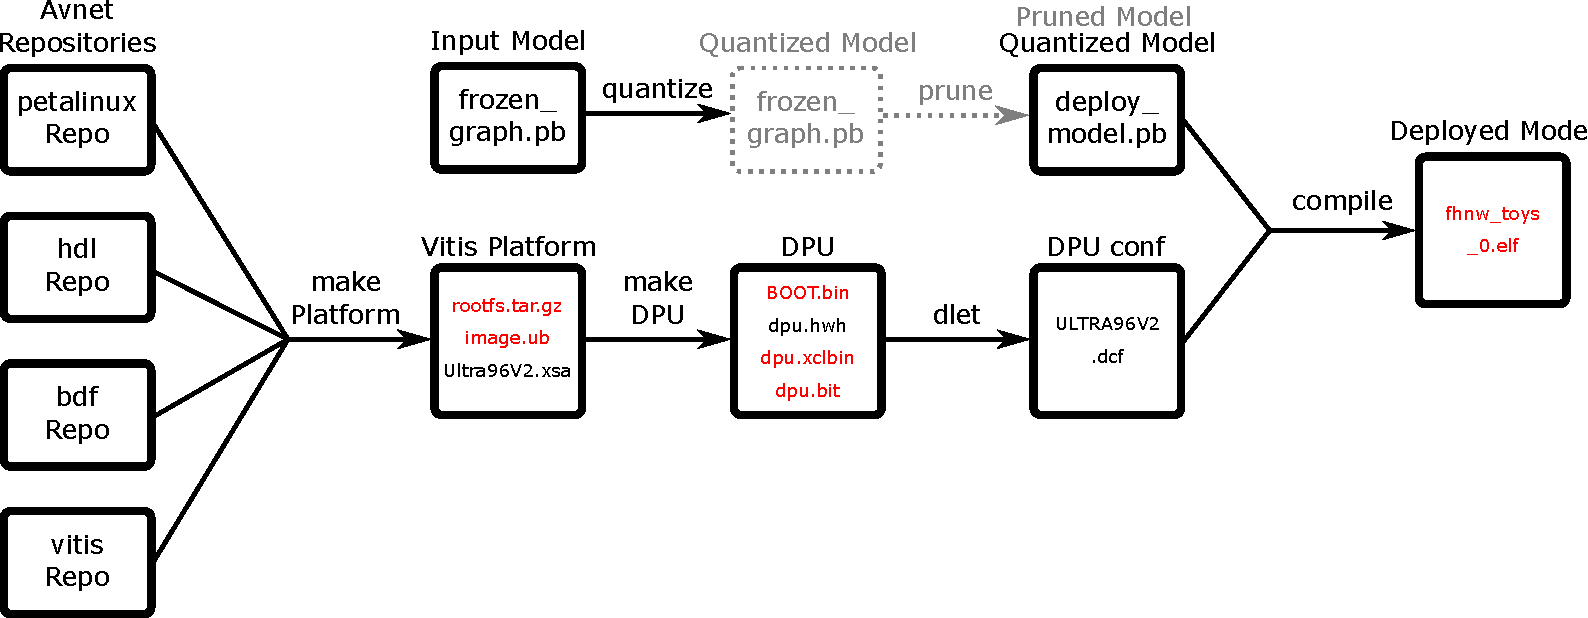
\includegraphics[width=1\textwidth]{graphics/workflow.pdf}
  \caption{PetaLinux workflow}
  \label{fig:petalinux_workflow}
\end{figure}

\paragraph{Build own Vitis Platform}
Four repositories from Avnet are required:
\begin{itemize}
  \item \texttt{bdf}
  \item \texttt{hdl}
  \item \texttt{petalinux}
  \item \texttt{vitis}
\end{itemize}

The \texttt{bdf} (board definition files) repository contains one folder for each of their development boards.
The \texttt{hdl} repo is required to use the \acrfull{pl} on UltraScale+ \acrshortpl{mpsoc}.
The \texttt{petalinux} archive contains, among other things, the configurations of the operating system PetaLinux.
To build a Vitis platform, the \texttt{vitis} archive is also required.
The \texttt{vitis} folder contains several Makefiles which refer to the other three repositories.
The repositories \texttt{hdl} and \texttt{petalinux} must be checked out to the same branch as the Xilinx Tools version.

The building process can be started with the Makefile in the \texttt{vitis/} directory.
Which board is used must be specified as a parameter.
Building the platform takes several hours, requires about \SI{200}{GB} of disk space and a minimum of \SI{32}{GB} of RAM.
After the process is completed, the platform is located in the \texttt{vitis/platform\_repo/} directory.

The Makefile from Avnet creates a sysroot by default.
Since all header and library files are included in this directory structure, cross compiling an application is possible.

\paragraph{Configure own Vitis Platform}
The platform can be adapted to individual needs.
First, a new PetaLinux project is created.
The generated directory \texttt{project-spec/meta-user} contains recipes for adding or removing programs like \acrshort{opencv} or a package manager.
Own recipes can be created with the command \texttt{petalinux-create -t apps}.
It is possible to create a component from existing content or from a predefined application template \cite{petalinux_commandline_guide}.

After adding all recipes, the commands \texttt{petalinux-config} and \texttt{petalinux-build} create the custom root filesystem, the required boot files and the Linux kernel \cite{petalinux_user_guide}.

The first stage bootloader, the device tree blob and U-Boot are stored in the \texttt{BOOT.BIN} file by default configuration.
They are required to initialize the board and load the kernel image \cite{xilinx_wiki_boot}.
The kernel image is located in the \texttt{image.ub} file \cite{xilinx_wiki_uboot}.
Both files are located in the \texttt{petalinux/projects/ultra96v2\_oob\_2019\_2/images/linux/} directory.

\paragraph{Flash SD Card}
The first step is to create the partitions for the boot files and for the root filesystem.
For the boot partition the format should be FAT32, while the root filesystem partition should be Ext4.
A space of \SI{1}{GB} for the boot partition is sufficient.
Furthermore, the boot label should be set for the boot partition.
In a next step, the created partitions must be formatted.
In a shell script it can be done as follows:

\begin{lstlisting}[style=bash, caption={Prepare SD card}, label=lst:create_partitions]
  DISK=/dev/sdb
  PART=

  # Create partitions
  sudo parted $DISK -s mkpart primary fat32 1MiB 1025MiB
  sudo parted $DISK -s mkpart primary ext4 1026MiB 100%

  # Set boot label
  sudo parted $DISK -s set 1 boot on

  # format partitions
  sudo mkfs -t vfat -F 32 -n boot $DISK${PART}1
  sudo mkfs -t ext4 -L rootfs $DISK${PART}2
\end{lstlisting}

The SD card is now ready to save the \acrshort{os}.
The files \texttt{BOOT.BIN} and \texttt{image.ub} can be copied to the boot partition and the \texttt{rootfs.tar.gz} file can be extracted to the rootfs partition.

\paragraph{Setup}
To use the \acrshort{dpu}, the \acrshort{n2cube} library is required.
This can either be added as a recipe when creating the operating system, or the header, include and library files can be copied manually afterwards.
The required files are available in the Docker image from Xilinx in the \texttt{/opt/vitis\_ai/xilinx\_vai\_board\_package/} directory.
The use of Docker and Xilinx is described in section \ref{sec:embedded_platform:model_deployment}.
The following files must be copied from the \texttt{xilinx\_vai\_board\_package/} directory:
\begin{itemize}
  \item \texttt{pkgs/bin/*} into the \texttt{/usr/local/bin/} directory of the board
  \item \texttt{pkgs/lib/*} into the \texttt{/usr/local/lib/} directory of the board
  \item \texttt{pkgs/include/*} into the \texttt{/usr/local/include/} directory of the board
\end{itemize}

Since \texttt{user/local/lib/} is not a default path for dynamic libraries, a \texttt{.conf} file must be created in the \texttt{/etc/ld.so.conf.d/} directory.
This file contains the path to the previously added libraries.
For example, the file could be named \texttt{dnndk.conf}, and its contents could look like this:
\begin{lstlisting}[style=bash, caption={}, label=lst:dnndk_conf_content]
  /usr/local/lib
\end{lstlisting}
Running \texttt{ldconfig} configures the dynamic loader to search for the \acrshort{n2cube} library in the \texttt{/usr/local/lib/} directory.
\texttt{ldconfig} is always executed at boot time.

To use the Baumer camera, the same procedure must be performed.
The respective include, library and header files can be obtained from Baumer.
